\chapter{Implementation, Integration and Test Plan}
\section{Overview}
In this section we will focus on steps to be conducted for the implementation, integration and test plan. 
Firstly, we ensure all the single units are created and tested on their own. Then we combine these unary modules into clusters that will perform a specific software sub-function. This will allow us to start the integrated testing of this clusters and test the interfaces between the units. This is crucial since the logic implemented in the modules differ from developer to developer. So, by testing them we ensure they work properly, and in case it allows us to detect possible errors in the interfaces. This process is repeated clustering the new formed units, until we reach the end.
The software integration test is to be repeated again several times to ensures that no new previously undetected errors spawn. It serves also to ensure that the correct performance level is reached.

\section{Integration testing approach:}
The approach chosen to the integration testing is the bottom-up one. It starts testing from the lowest unit of the application and gradually moves towards integrating and testing the upper ones until all the units are integrated as one. Then the system as whole is tested. This process require the use of drivers that are disposable components made ad hoc to be placed on a higher level of the component tested to call their function. 
This approach was chosen because it allows us to localize in an easier way the possible errors in the lower levels, where is present the most complex component, the scheduler. The approach divides the component in five ordered blocks.\\

\begin{figure}[H]
    \centering
    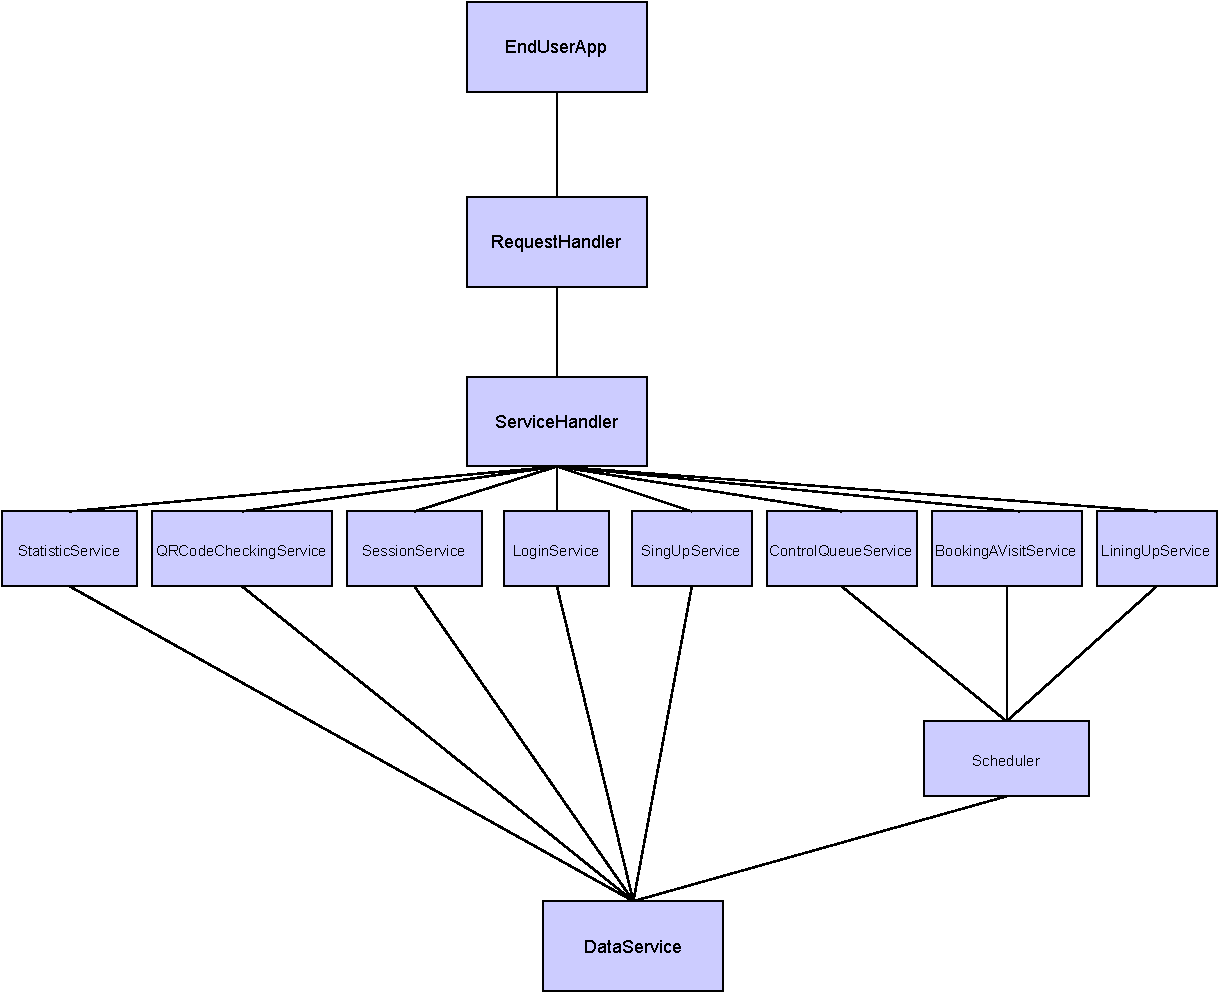
\includegraphics[width=1.0\textwidth]{images/component_hierarchy.pdf}
    \caption{hierarchy of components.}
\end{figure}

As shown in the hierarchy of the components, the lowest component of the system and so the first one to be tested and implemented is the DataService. Every other component directly or not, rely on this one since they require to store and retrieve data to function. On the other hand, the data service does not rely on other components and so it can function in isolation. \\
The Scheduler should be implemented next and so as second block, since it is the most complex system of the bottom level ones that use different component to function. Its function is to schedule both statically and dynamically for the app users, the order of their turn in the queue. It requires to consider both people that lined up and booked a visit, and possibly their data and position. It also ineteracts through the FireBaseService with the app-users to notify them when it is their turn.
Inside the scheduler the first component to be implemented is the StaticSchedulingService. Since it is the one that handles first the request from the higher level and could function independently of the DynamicScheduler. It requires to build the drivers of the basic function of the upper modules and the integration with GoogleMapsServices and GroceryStoreService. After that the DynamicScheduler has to be implemented starting from the AlertService and a drive of the QueueManager to verify that the notification request are sent correctly to the GoogleFireBaseService. Then QueueManagerService and UserPositionService can be implemented and integrated in parallel. \\
The third block commence after the start of the implementation of the scheduler, the component to be integrated in parallel or immediately following are the StatisticService, QRCodeCheckingSerivice, LoginService, SingUpService and SessionService. Since all of them work independently to each other their order is also interchangeable, but the order of implementation chosen is the following:
The first one is StatisticService, it offers function to the store manager and it is not strictly bond with the client interface. The second and third are LoginService and SingUpService, one serves to allow user to login and the other to allow user to sign in. The fourth one checks that the information scanned by the turnstile are correct and match the ones in the database. The last one, SessionService manages the session of the different users and so it more dependent on the higher levels. All of them require the use and so the develop of a driver of the ServiceHandler. \\
Subsequently the fourth block begin, after the scheduler is integrated, the component to implements are ControlQueueService, BookingAVisitService and LiningUpService. All of them need a driver for the ServiceHandler and must interact with the scheduler. The first one to change parameters and block the release of the new tickets, the second and third ones allow user to get respectively booking ticket and lining up ticket. The BookingAVisitService permits also to insert more information about the visit while the LiningUpService has also to check the user type to decide to monitor their position. The order of implementation of this block of component is the following: First the LiningUpService since it is the most important of the three then BookingAVisitService and lastly the ControlQueueService because it will be easier to check if it works as expected if the LiningUpService is already implemented. \\
And in the end the last block to be integrated is composed in order of the ServiceHandler, RequestHandler and the EndUserApp. The order of integration is clear since they are in different levels, it require to develop the RequestHandler and then EndUserApp drivers when proceeding on the implementation. 
Since they are the last ones to be implemented the testing should be done more meticulously to ensure that the almost complete system works as thought. Especially because these components are crucial to its functioning, they allow so send the request from the device, elaborate them and redirect on the right component.\\
The interfaces of the hardware component of the store and so turnstile, scanner and printer are included in the GroceryStoreSerivice. And so even though they are already implemented and tested, they should by further tested on site to verify that the acquisition of data, the output data and the state transition are correct. 
\begin{figure}[H]
    \centering
    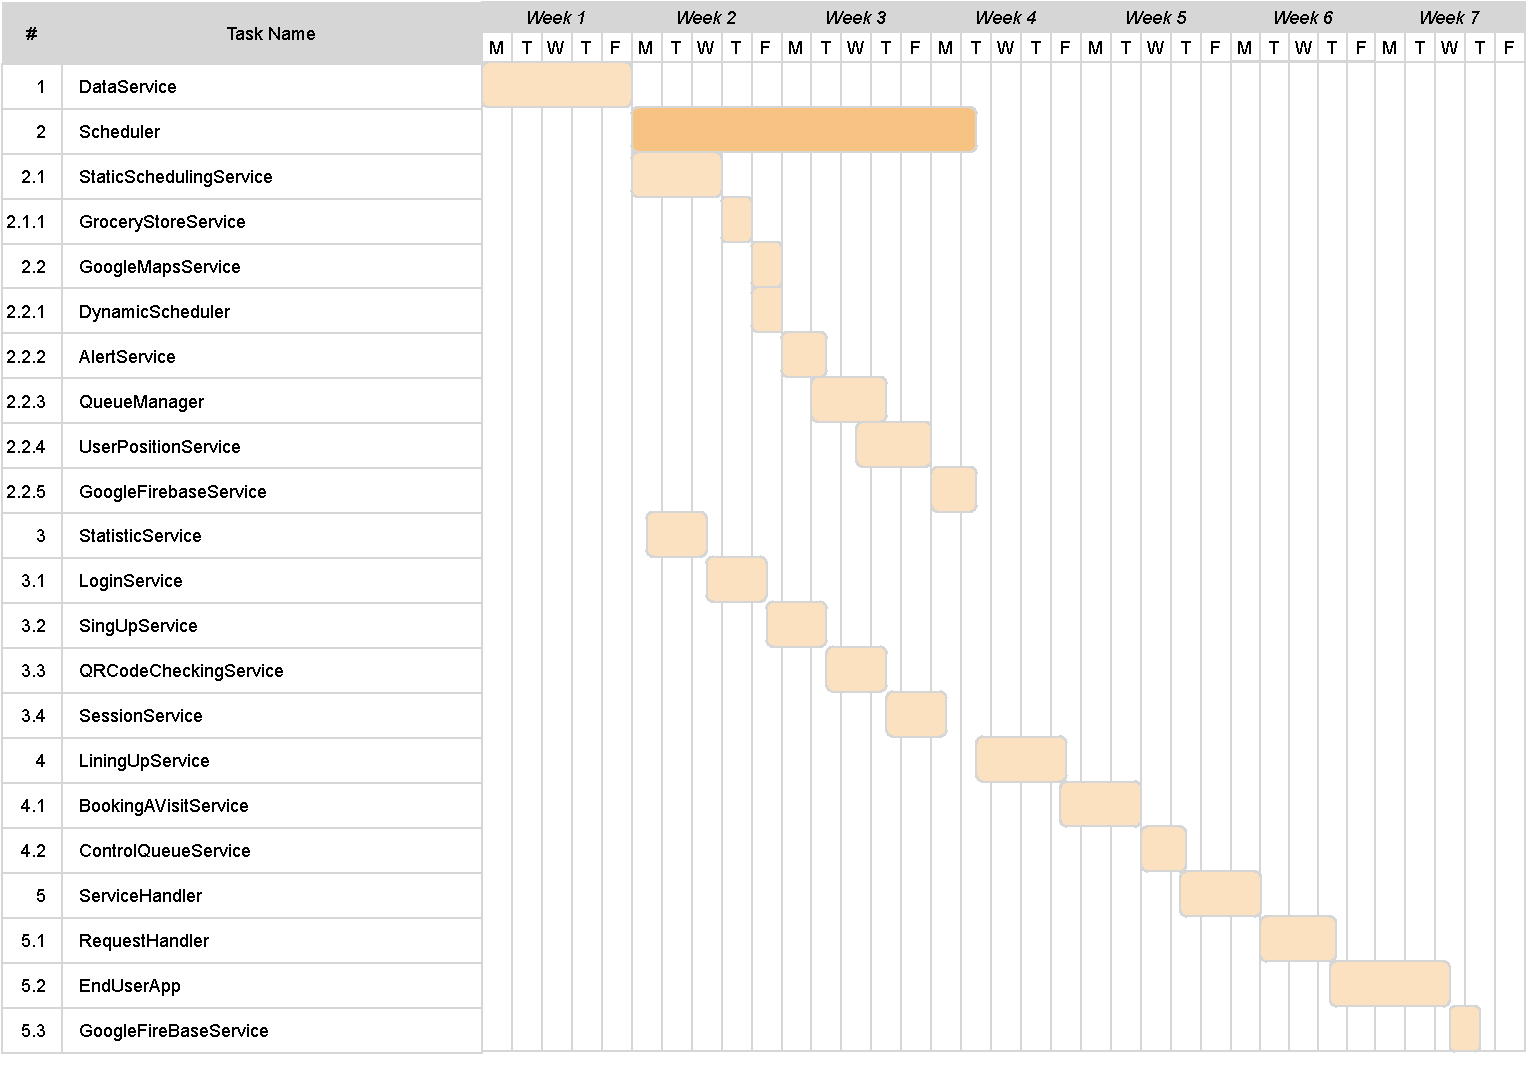
\includegraphics[width=1.0\textwidth]{images/Gantt.pdf}
    \caption{Gantt chart.}
\end{figure}

\section{Integration strategy :}
As stated in the previous section,the approach chosen it the bottom-up one so the first component to be unit tested is the DataService. After it is implemented on top of that the scheduler and a driver to simulate the inputs.
\begin{figure}[H]
    \centering
    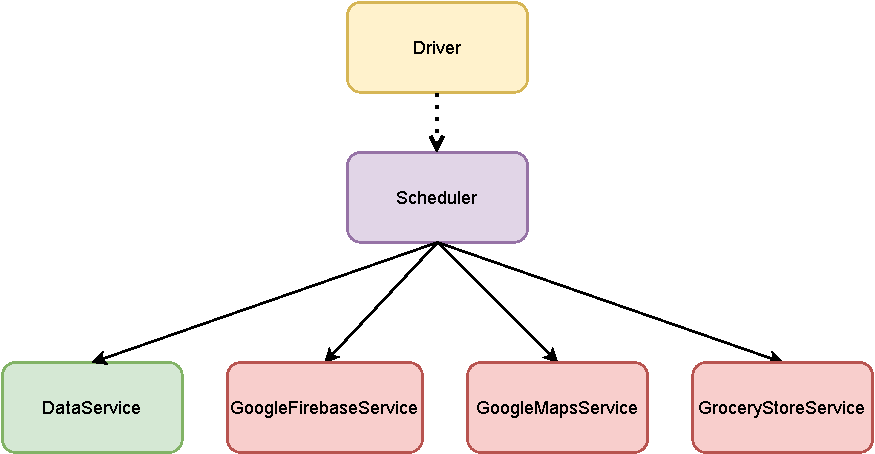
\includegraphics[width=1.0\textwidth]{images/component1.pdf}
    \caption{Integration step 1.}
\end{figure}
The scheduler being a complex component includes first the implementation of the StaticSchedulingService with the DataService and the two external services. Next the AlertService has to be implemented with GoogleFirebaseService
\begin{figure}[H]
    \centering
    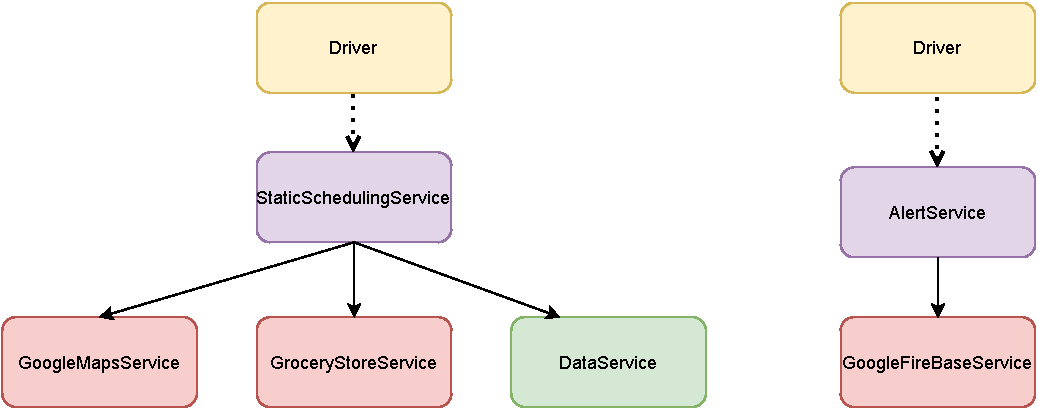
\includegraphics[width=1.0\textwidth]{images/component2.pdf}
    \caption{Integration step 2.}
\end{figure}
Then the QueueManagerService is implemented and integrated with the StaticSchedulingService and AlertService. Which causes the merge of the two small clusters.
\begin{figure}[H]
    \centering
    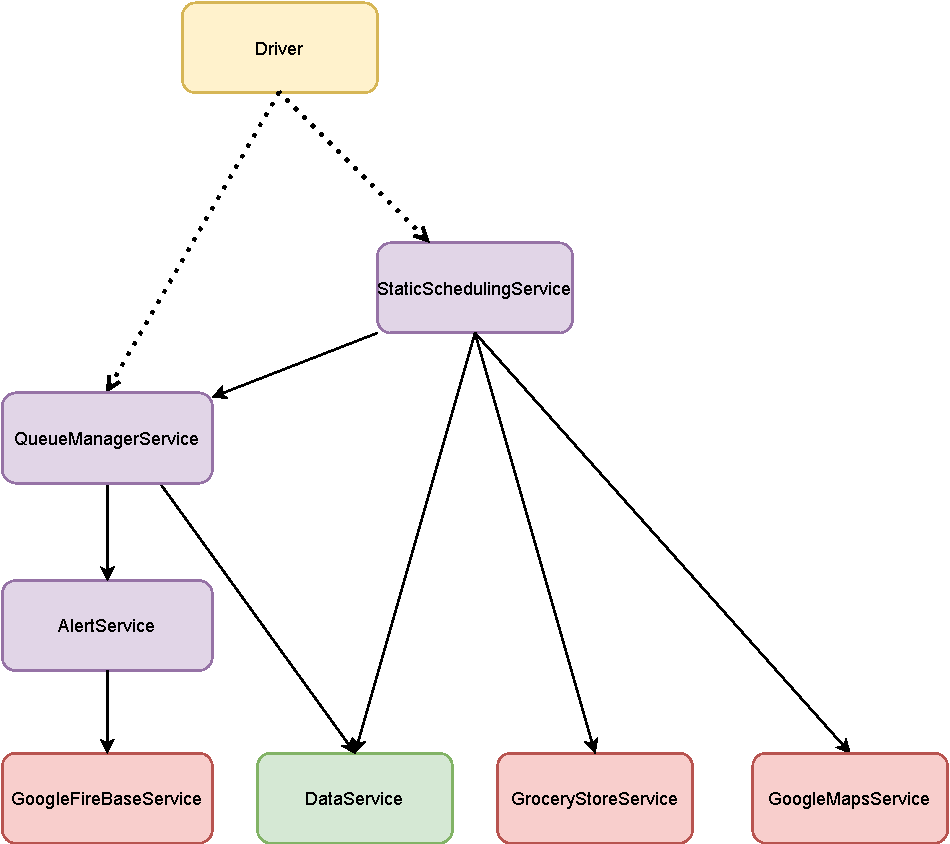
\includegraphics[width=1.0\textwidth]{images/component3.pdf}
    \caption{Integration step 3.}
\end{figure}
The UserPositionSerivice is implemented for last inside the scheduler and it completes it.
\begin{figure}[H]
    \centering
    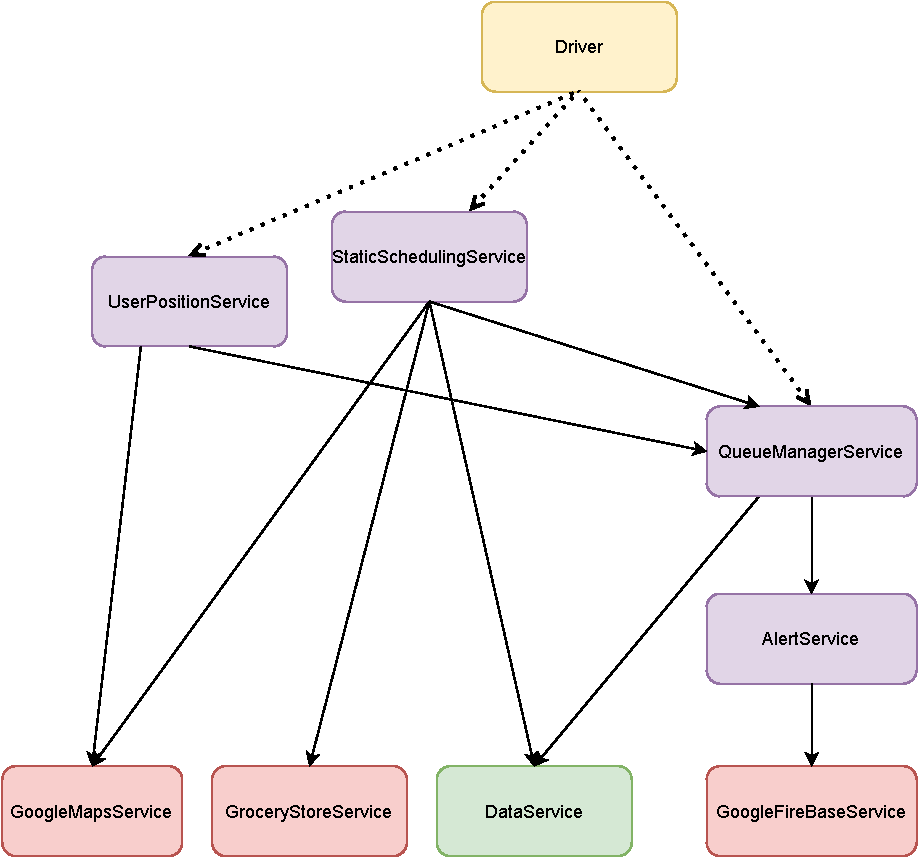
\includegraphics[width=1.0\textwidth]{images/component4.pdf}
    \caption{Integration step 4.}
\end{figure}
Simultaneously the components StatisticService, LoginService, SignUpService, QRCodeCheckingService and SessionService are implemented on the DataService in this order,with a driver of the ServiceHandler.
\begin{figure}[H]
    \centering
    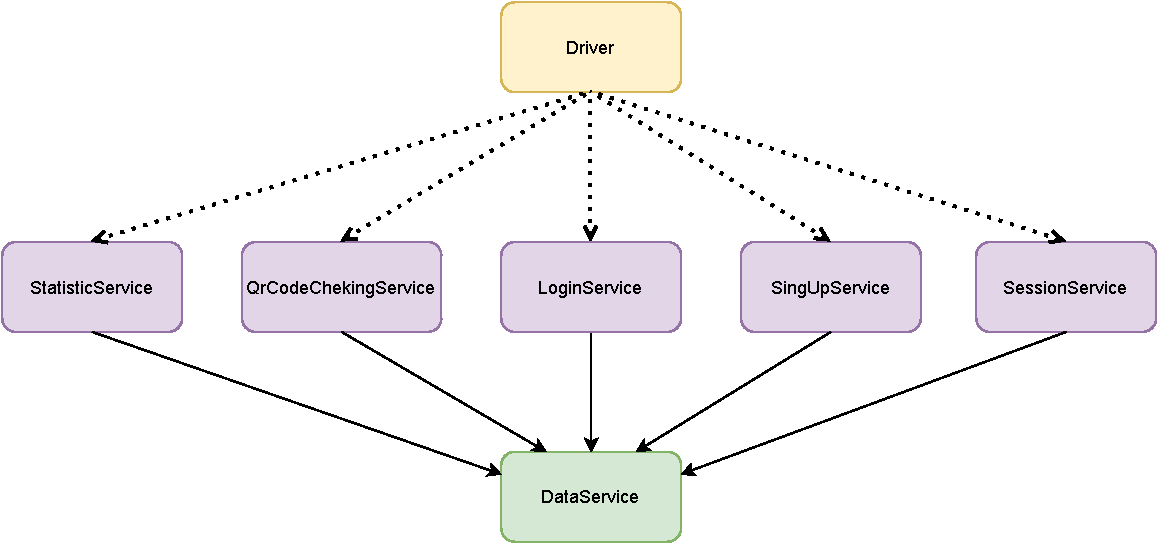
\includegraphics[width=1.0\textwidth]{images/component5.pdf}
    \caption{Integration step 5.}
\end{figure}
After the integration of the scheduler, the components that are implemented on top are in order LiningUpService, BookingAVisitService, ControlQueueService.
\begin{figure}[H]
    \centering
    \includegraphics[width=1.0\textwidth]{images/component6.pdf}
    \caption{Integration step 6.}
\end{figure}
Lastly, the component implemented are the ServiceHandler with the driver on top, then the RequestHandler with the driver and finally the EndUserApp with the GoogleFirebaseService.
\begin{figure}[H]
    \centering
    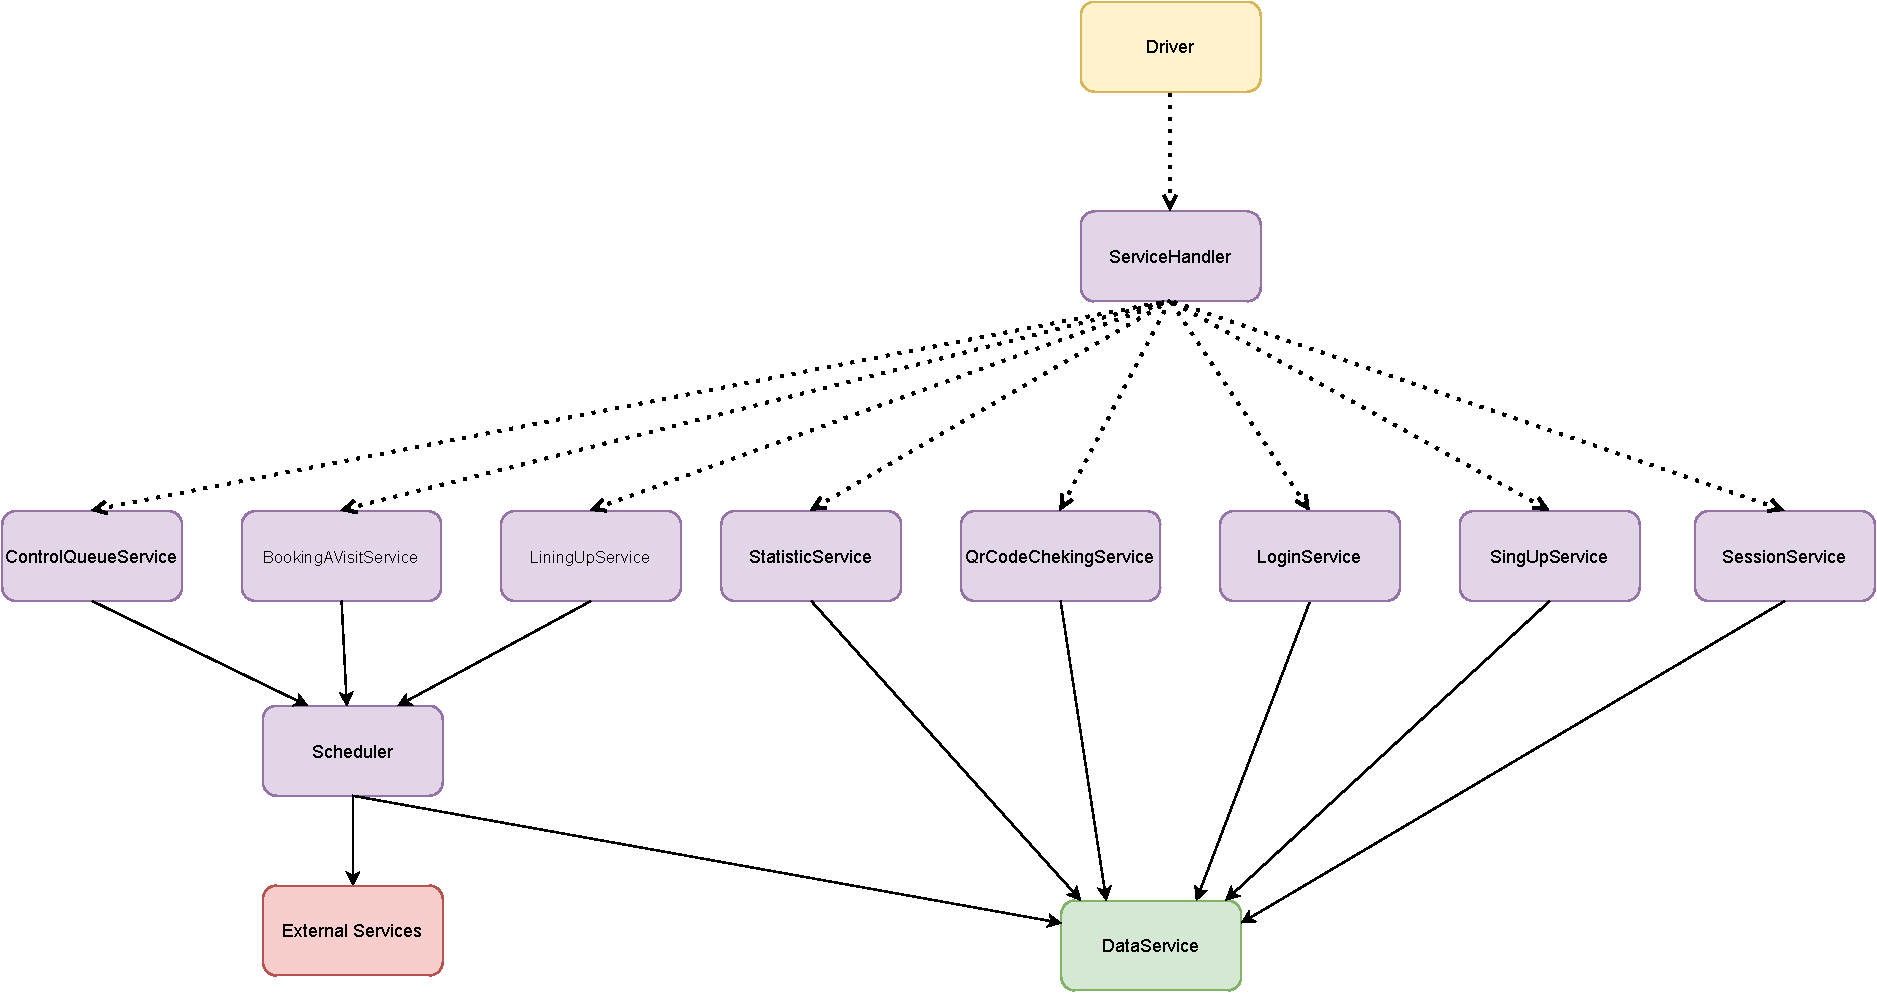
\includegraphics[width=1.0\textwidth]{images/component7.pdf}
    \caption{Integration step 7.}
\end{figure}
\begin{figure}[H]
    \centering
    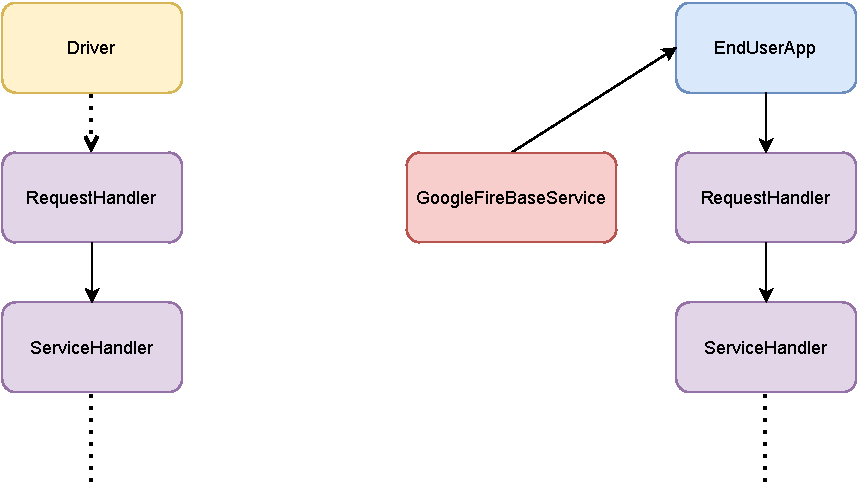
\includegraphics[width=1.0\textwidth]{images/component8.pdf}
    \caption{Integration step 8.}
\end{figure}
